% !TEX root = lecture/Differential_Geometry.tex

% \tikzset{external/export=false}
\begin{definition}
    $ \dd N_p $ has eigenvector  $ e_1,e_2 $ and 
    \[\dd N_p(e_1)=-k_1e_1,\,\dd N_p(e_2)=-k_2e_2\]
    Then  $ k_1,k_2 $ is called the \name{principal curvature} of  $ S $ at  $ p $,  $ e_1,e_2 $ is called the \name{principal directions} of  $ S $ at  $ p $.       
\end{definition}

\begin{definition}
    If  $ k_1,k_2  $ is the principal curvatures of  $ S  $ at  $ p $, $ N_p $ is the Gauss map,  then the \name{Gaussian curvature} is  $ K=\det \dd N_p=k_1k_2 $. The \name{average curvature}   $ H=-\dps\frac{1}{2}\tr \dd N_p=\frac{1}{2}(k_1+k_2) $. 
\end{definition}
\begin{example}
    For a cylinder  $ \{(x,y,z)|x^2+y^2=1\} $,  $ N(p)=(-x,-y,0) $,  $ \dd N_p=(-x'(p),-y'(p),0) $. So  $ k_1=0,k_2=1,K=0 $.    
\end{example}
\begin{example}
    $ S=\{z=y^2-x^2\}\subset \Rbb^2 $.  $ \dd N=\dps\frac{1}{\sqrt{4u^2+4v^2+1}}(2u,-2v,1) $. Then  $ k_1=2,k_2=-2,K=-4<0 $.   
\end{example}

\begin{center}
    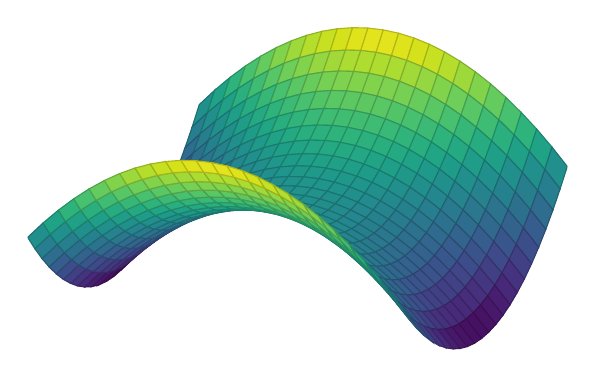
\begin{tikzpicture}
        \begin{axis}[    
            axis lines = none,       % 设置坐标轴通过原点
            xlabel = {$x$},            % x轴标签
            ylabel = {$y$},            % y轴标签
            zlabel = {$z$},            % z轴标签
            % title = {$z = y^2-x^2$},  % 图像标题
            % title style={at={(0.5,-0.1)}, anchor=north},
            colormap/viridis,          % 选择颜色映射
            ]
            \addplot3[
                surf,                    % 使用表面绘图
                domain=-3:3,              % x和y的范围
                y domain=-3:3,
            ]
            {y^2-x^2};    % 目标函数 z = sin(x^2 + y^2)
        \end{axis}
    \end{tikzpicture}
\end{center}
\begin{definition}
    For  $ p\in S $ in a surface,
    
    Call it  \name{elliptic} if  $ \det \dd N_p>0 $.
    
    Call it \name{hyperbolic} if  $ \det \dd N_p<0 $. 
    
    Call it \name{parabolic} if  $ \det \dd N_p=0 $ but  $ \dd N_p\neq 0 $, or call it \name{planar} if  $ \dd N_p=0 $.   
\end{definition}

The 1st fundamental form $ \Romannumer1_p=E\dd u^2+2F\dd u\dd v+G\dd v^2 $ where 
\begin{equation}
    E=\<X_u,X_u\>,\,F=\<X_u,X_v\>,\,G=\<X_v,X_v\>
\end{equation} 

However,
$ \Romannumer2(\alpha')=e\dd u^2+2f\dd u\dd v+g\dd v^2 $ where
\begin{equation}
    e=\<N,X_{u,u}\>,\, f=\<N,X_{u,v}\>,\, g=\<N,X_{v,v}\>
\end{equation} 

Since  $ \{X_u,X_v, N\} $ is an orthogonormal basis in  $ \Rbb^3 $,  $ \<N,N\>=1 $  $ \Rightarrow  $  $ 2\<N_u,N\>=0 $ if we take  $ \dps\frac{\partial }{\partial u} $. Then 
\[\begin{cases}
    N_u=a_{11}X_u+a_{21}X_v\\
    N_v=a_{12}X_u+a_{22}X_v
\end{cases}\]  
Then for  $ \dd N(\alpha')=\dd N(X_u\cdot u'+X_v\cdot v')=\begin{pmatrix}
    a_{11}&a_{12}\\
    a_{21}&a_{22}
\end{pmatrix}\cdot\begin{pmatrix}
    u'\\
    v'
\end{pmatrix}$. Therefore,  $ \dd N=\begin{pmatrix}
    a_{11}&a_{12}\\
    a_{21}&a_{22}
\end{pmatrix} $. Now 
\[f=\<N,X_{u,v}\>=-\<N_v,X_u\>=-\<a_{12}X_u+a_{22}X_v,X_u\>=-a_{12}E-a_{22}F\]
Similarly, one can prove 
\[f=-\<N_v,X_u\>=-a_{12}E-a_{22}F\]
\[e=-\<N_u,X_u\>=-a_{11}E-a_{21}F\]
\[g=-\<N_v,X_v\>=-a_{12}F-a_{22}G\]

So 
\[-\begin{pmatrix}
    e&f\\
    f&g 
\end{pmatrix}=\begin{pmatrix}
    a_{11}&a_{12}\\
    a_{21}&a_{22}   
\end{pmatrix}\begin{pmatrix}
    E&F\\
    F&G
\end{pmatrix}\]
 $ \Rightarrow  $ 
\begin{equation}
    \begin{pmatrix}
        a_{11}&a_{12}\\
        a_{21}&a_{22}
    \end{pmatrix}=-\frac{1}{EG-F^2}\begin{pmatrix}
        e&f\\
        f&g
    \end{pmatrix}\begin{pmatrix}
        G&-F\\
        -F&E
    \end{pmatrix}
\end{equation} 
\ie 
\begin{equation}
    \begin{aligned}
        &a_{11}=\frac{fF-eG}{EG-F^2}&a_{12}=\frac{gF-fG}{EG-F^2}\\
        &a_{21}=\frac{eF-fE}{EG-F^2}&a_{22}=\frac{fE-gE}{EG-F^2}
    \end{aligned}
\end{equation}
So  $ K=\det \dd N_p=\dps\frac{eg-f^2}{EG-F^2} $,  $ H=-\tr \dd N_p=\dps\frac{1}{2}\cdot\frac{eG-2fF+gE}{EG-F^2}$. 

\begin{example}
    For torus  $ T^2=S^1\times S^1 $, 
    
    $ X(u,v)=((a+r\cos u)\cos v,(a+r\cos u)\sin v,r\sin u) $.

    Then we can calculate  $ E,F,G,N $ by calculating  $ X_u,X_v $. And we obtain  $ f,g,e $ in a similar way. The result 
    \[K=\frac{eg-f^2}{EG-F^2}=\frac{\cos u}{r(a+r\cos v)}\]  
    Then 
    \[\begin{cases}
        K=0&u=\dps\frac{\pi}{2}\text{ or }\frac{3\pi}{2}\\
        K<0&\dps\frac{3\pi}{2}>u>\frac{\pi}{2}\\
        K>0&\text{otherwise}
    \end{cases}\] 

    So the torus is elliptic in the outer half and is hyperbolic in the inner half. 

    \begin{center}     
        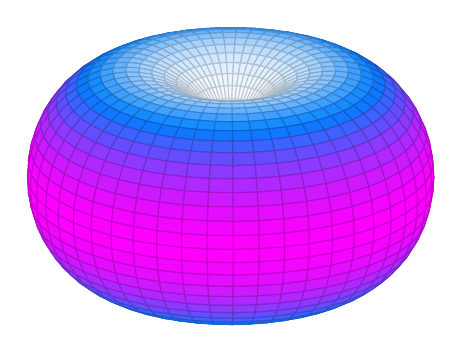
\begin{tikzpicture}
            \begin{axis}[
                axis lines = none,
            ]
                \addplot3[surf,
                colormap/cool,
                samples=50,
                domain=0:2*pi,y domain=0:2*pi,
                z buffer=sort,
                point meta={x * x + y * y}
                ]
               ({(2 + 2 * cos(deg(x))) * cos(deg(y + pi/2))}, 
                {(2 + 2 * cos(deg(x))) * sin(deg(y + pi/2))}, 
                {2 * sin(deg(x))});
            \end{axis}
        \end{tikzpicture}
    \end{center}
    
\end{example}

\begin{theorem}[Gauss Theorem Egregium]\label{Gauss fantanstic theorem}
    $ K  $ is the invariant of  $ S $, only depending on  $ E,F,G $.  Equivalently, Gauss curvature is invariant under local isometry.
\end{theorem}
\begin{proof}
    For  $ \{X_u,X_v,N\} $ an orthogonormal basis of  $ \Rbb^3 $, let 
    \[X_{u,u}=\Gamma^1_{11}X_u+\Gamma_{11}^2X_v+L_1N\]
    \[X_{u,v}=\Gamma_{12}^1X_u+\Gamma_{12}^2X_v+L_2N\]  
    \[X_{v,u}=\Gamma_{21}^1X_u+\Gamma_{21}^2X_v+\tilde{L}_2N\]
    \[X_{v,v}=\Gamma_{22}^1X_u+\Gamma_{22}^2X_v+L_3N\]
    where  $ \Gamma_{ij}^k $ is called \name{Cristopher symbol},  $ \Gamma_{21}^i=\Gamma_{21}^i,i=1,2 $ 
    \[N_u=a_{11}X_u+a_{12}X_v\]
    \[N_v=a_{12}X_u+a_{22}X_v\]
    Then take the inner product of  $ X_{u,u} $ with  $ N,X_u,X_v $ separately  
    \[e=\<X_{u,u},N\>=L_1\]
    \[\frac{1}{2}E_u=\frac{1}{2}\cdot\frac{\partial }{\partial u}\<X_u,X_u\>=\<X_{u,u},X_u\>=\Gamma_{1,1}^1E+\Gamma_{12}^2F\]
    \[F_u-\frac{1}{2}E_v=\<X_{u,u},X_v\>=\Gamma_{11}^1F+\Gamma_{11}^2G\]
    So we have  $ \begin{cases}
        L_1=e\\
        \Gamma_{11}^1E+\Gamma_{11}^2F=\dps\frac{1}{2}E_u\\
        \Gamma_{11}^1F+\Gamma_{11}^2G=\dps\frac{1}{2}F_u-\frac{1}{2}E_v
    \end{cases} $ \ie 
    \begin{equation}
        \begin{pmatrix}
            \Gamma_{11}^1\\
            \Gamma_{11}^2
        \end{pmatrix}=\begin{pmatrix}
            E&F\\
            F&G
        \end{pmatrix}^{-1}\begin{pmatrix}
            \dps\frac{1}{2}E_u\\
            F_u-\frac{1}{2}E_v
        \end{pmatrix}
    \end{equation}
    So any  $ \Gamma_{ij}^k $ can be represented by  $ E,F,G $.
    
    Now since   $ (X_{u,u})_v=(X_{v,v})_u $.
    
    \begin{equation}
        \begin{aligned}
            \frac{\partial }{\partial v}X_{u,u}&=((\Gamma_{11}^1)_vX_u+\Gamma_{11}^1X_{uv})+((\Gamma_{11}^2)_vX_v+\Gamma_{11}^2X_{vv})+((e_1)_vN+eN_v)\\
            &=(\Gamma_{11}^1)_vX_u+\Gamma_{11}^1((\Gamma_{12}^1)X_u+\Gamma_{12}^2X_v+fN)\\
            &+(\Gamma_{11}^2)_vX_v+\Gamma_{11}^2(\Gamma_{22}^1X_u+\Gamma_{22}^2X_v+gN)\\
            &+e_vN+e(a_{12}X_u+a_{22}X_v)
        \end{aligned}
    \end{equation}
    Similarly, one can calculate that
    \begin{equation}
        \begin{aligned}
            \frac{\partial}{\partial u}X_{u,v}&=(\Gamma_{12}^1)_uX_u+\Gamma_{12}^1(\Gamma_{11}^1X_u+\Gamma_{11}^2X_v+eN)\\
            &+(\Gamma_{12}^2)_uX_v+\Gamma_{12}^2(\Gamma_{12}^1X_u+\Gamma_{12}^2X_v+fN)\\
            &+f_uN+f(a_{11}X_u+a_{21}X_v)
        \end{aligned}
    \end{equation}
    The coefficients of  $ X_v $ is 
    \[\Gamma_{11}^1\Gamma_{12}^2+(\Gamma_{11}^2)_v+\Gamma_{11}^2\Gamma_{22}^2+ea_{22}=\Gamma_{12}^1\Gamma_{11}^2+(\Gamma_{12}^2)_u+\Gamma_{12}^2\Gamma_{12}^2+fa_{21}\]
    where 
    \[ea_{22}-fa_{21}=\frac{(efF-egE)-(feF-f^2E)}{EG-F^2}=\frac{(f^2-eg)E}{EG-F^2}=-KE\]
    So we obtain
    \begin{equation}
        \frac{(\Gamma_{11}^1\Gamma_{12}^2+(\Gamma_{11}^2)_v+\Gamma_{11}^2\Gamma_{22}^2)-(\Gamma_{12}^1\Gamma_{11}^2+(\Gamma_{12}^2)_u+\Gamma_{12}^2\Gamma_{12}^2)}{E}=K
    \end{equation} 

    Here we have proved that  $ K  $ can be represented by  $ E,F,G $.
\end{proof}

This is the \name{Gauss formula} we obtain 
\begin{equation}\label{Gauss equation 1}
    (\Gamma_{12}^2)_u-(\Gamma_{11}^2)_v+\Gamma_{12}^1\Gamma_{11}^2+\Gamma_{12}^2\Gamma_{12}^2-\Gamma_{11}^2\Gamma_{22}^2-\Gamma_{11}^1\Gamma_{12}^2=-EK
\end{equation}

Similarly, one can prove for the coefficients of  $ X_u $
    \begin{equation}\label{Gauss equation 2}
        (\Gamma_{12}^1)_u-(\Gamma_{11}^1)_v+\Gamma_{12}^2\Gamma_{12}^1-\Gamma_{11}^2\Gamma_{22}^1=FK
    \end{equation}
It is (when  $ F\neq 0 $) merely another form of the Gauss formula.

    And the coefficients of  $ N $
    \begin{equation}\label{Gauss equation 3}
        e_v-f_u=e\Gamma_{12}^1-f(\Gamma_{12}^2-\Gamma_{11}^1)-g\Gamma_{11}^2
    \end{equation} 

By applying the same process  to  $ (x_{v,v})_u=(x_{u,v})_v $, we obtain the equation giving again the
Gauss formula \eqref{Gauss equation 1}. Furthermore, we can obtain another equation 

\begin{equation}\label{Gauss equation 4}
    f_v-g_u=e\Gamma_{22}^1+f(\Gamma_{22}^2-\Gamma_{12}^1)-g\Gamma_{12}^2        
\end{equation}
\eqref{Gauss equation 3} and \eqref{Gauss equation 4} are called \name{Maindardi-Codazzi} equations

The Gauss formula and the Mainardi-Codazzi equations are known under the name of compatibility equations of the theory of surfaces.
\begin{theorem}
    If  $ E,F,G,e,f,g $ satisfies \eqref{Gauss equation 1}  $ \sim $  \eqref{Gauss equation 4}, then it uniquely determines a surface.
\end{theorem}
% \tikzset{external/export=true}